\chapter{Design and Implementation}
\label{design}

This section presents the design of the FPGA-based control board prototype. The design followed the top-down design stages of the V-model shown in Figure \ref{V-model}. This section follows the design flow by first discussing the requirements for the system and how they were identified. This includes the identification of the subset of requirements necessary to implement the safety function of the device. This is followed by a presentation of the architecture that was derived from these requirements. The design and implementation of the modules which form the architecture is then presented. The physical prototype, created as part of this project, is then discussed.

\section{V-Model Design Process}

%The V-model is an iterative methodology which promotes...

The design stages outlined in the V-model follow a top-down methodology. The methodology starts with the definition of the system and safety requirements.
From these requirements, an architecture is derived.
The behaviour of this architecture must then be modelled. 
Modules which form the architecture can then be designed.
The final stage of design, following the V-model, is the synthesis, placement and routing of the design. This stage involves the application of constraints to the synthesis environment as well as the mapping of the design.
Each of these activities are described in the following sections.


%The major focus of the V-model is on the verification of the design on every level. In order to achieve this, the system must be designed for testability. For example, on a module level, modules should be well contained, simple and have well-defined functionality. The reuse of modules also reduces the verification effort. 


\section{Prototype System Requirements}

An ATyS specification document was created by Socomec as part of a previous iteration of the device. 
% original ATyS requirements
This existing specification of the microcontroller-based system represents a full set of the requirements for the ATyS motor control. The motor control process has a number of operating modes and possible conditions. This includes the option to change the load motor as well as the command interface. For example, the commands can come from a customer input or from the source detection board of the ATyS. 


%\subsection{Prototype Scope and Safety Requirements}

For this prototype, the requirements which are necessary for performing the motor control were identified and this became the specification for the prototype.
Only safety features should be considered with respect to the functional safety of the device\cite{HayekSRAM}.
% requirements specification process - move this process to the safety requirements section?
The comprehensive microcontroller specification was used to derive the subset of requirements to be implemented as a prototype. The motor control process was identified as the safety function and so this was the central focus for the prototype design. It is the core behaviour of the device and performs the essential behaviour of changing the connection from one source to another. External PCB requirements are outside of the scope of this project. Only the motor control requirements that relate to the processor and its interfaces were considered for this design. The requirements for the prototype are outlined in Table \ref{requirements-table}.


%\subsection{Motor Control Process}

The overall process of motor control involves moving from the current position to a desired position and stopping when the position is reached. Several stages, which need to be performed in order to complete this process, are outlined in the existing specification. 
%The process begins with the driving of the required Thyristor and IGBT opposite pair (see Figure \ref{motor_control_circuit}). After this, a minimum PWM value is provided to the IGBTs. This value is increased until it reaches the maximum value and then the PWM duty-cycle is regulated based on the motor current. If the position is reached within five seconds, the motor is stopped. However; if the desired position is not reached within five seconds, the cycle is repeated and if still not successful after a further five seconds, the device is put into an error state and a relay is driven.
%\subsection{Requirements for Performing Motor Control}
% the requirements of this project 
The external interfacing requirements of the motor control process can be broken down into three sections. The first of which is the command input. This uses a simple command which is input to the device by activating a number of pins. 
The second requirement is the constant detection of the position. This is done using a series of pushbuttons, the state of which determine the physical position of the motor. 
The final required interface of the motor control safety function is the control of the motor.  
There are also internal requirements for the processing of these inputs and outputs. 
PWM regulation allows for accurate motor control. The regulation scheme is to use the motor current value to adjust the PWM supply to the motor. PWM regulation also dependant on the supply voltage. 



\begin{table}[t]
\centering
\begin{tabular}{ |p{0.2\textwidth}|p{0.6\textwidth}| }
 \hline
 \multicolumn{2}{|c|}{ATyS Motor Control Requirements} \\
 \hline
 Requirement & Description \\
 \hline
 \hline

 Input R1 & Translate the three valid command inputs into an encoded format \\
 \hline 
 Input R2 & Translate the seven valid position inputs into an encoded format \\
 \hline 
 Input R3 & Calculate the direction of movement required based on the position and command inputs \\
 \hline 
 Input R4 & Control the motor movement stages: startup, regulation and braking \\
 \hline
 PWM R1 & Control the duty-cycle through each of the preset motor control stages \\
 \hline
 PWM R2 & Regulate the PWM based on the measured current value - limit to 1.5A \\
 \hline 
 PWM R3 & Generate a 1kHz PWM signal of a duty-cycle which is calculated by the regulation process \\
 \hline 
 PWM R4 & Update the current value in the middle of the PWM on-time \\
 \hline
 PWM R5 & Limit the maximum PWM based on the supply voltage (100\% below 170V and reducing linearly to 50\% at 333V) \\
 \hline
 ADC R1 & Measure the supply voltage to 8-bit resolution when the motor is not being operated \\
 \hline
 ADC R2 & Measure the motor current to 8-bit resolution when the motor is being operated \\
 \hline
 Drive R1 & Drive the IGBTs based on the control signals generated by the Input Processing module %(see Figure \ref{motor_control_circuit} below) 
 \\
  \hline
 Drive R2 & Drive the Thyristors based on the control signals generated by the Input Processing module \\
 \hline
\end{tabular}

\caption{List of requirements for performing the motor control safety-function of the ATyS}
\label{requirements-table}
\end {table}

%The PWM Regulation requirements, marked as PWM in Table \ref{requirements-table}, were only required for error cases. The regulation process would not need to run under normal conditions where

\section{System Architecture}

As dictated by the V-model process, the system architecture was derived from the system requirements. Similar FPGA implementations were analysed in order to identify common functional units used in FPGA motor control systems. Several architectures which have been designed in order to perform motor driving were analysed and common functional units include ADCs, position measurement, current regulation and PWM modules\cite{Jeppesen, MonmassonFPGABasedControllers, Dubey, Idkhajine, Aime}. Each of these units translates to the interfacing and processing requirements of the ATyS. The architecture which was derived from the requirements for this system is shown in Figure \ref{sys_architecture}. The inputs and outputs were defined by the requirements for accepting commands, reading position, analogue value monitoring and providing motor control signals. With a defined set of interfaces, the processes required in order to fulfil the requirements had to be decided. The system must make a decision based on the command and position inputs as to what motor control is required. The Input Processing module was added to the architecture in order to achieve this. The system must be able to measure the supply voltage and motor current in order to adjust the control scheme based on the environment. An ADC module was incorporated to provide these values to the regulation scheme.
In cases of a stalled or blocked motor, the system must control regulation on the current to prevent high currents. The PWM Regulation module takes the output from the Input Processing and the reading from the ADC in order to control the current. The PWM signal which is generated must be correctly routed to the motor control circuitry. The Motor Driving module was added to the architecture in order to achieve this. 


%\begin{figure}[h]
%\centering
%\includegraphics[width=0.95\textwidth]{images/SystemArchitecture.pdf}
%\caption{High-level system architecture diagram showing system processes}
%\label{system_architecture}
%\end{figure}

\begin{figure}
    \centering
    

\tikzset{every picture/.style={line width=0.75pt}} %set default line width to 0.75pt        

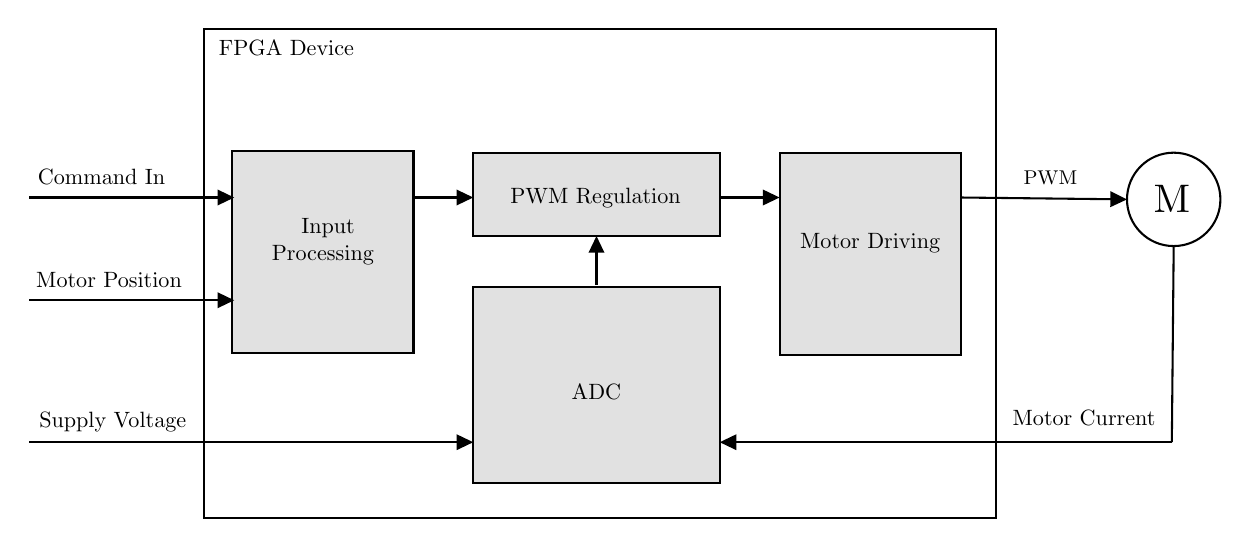
\begin{tikzpicture}[x=0.75pt,y=0.75pt,yscale=-0.9,xscale=0.9]
%uncomment if require: \path (0,290.6363525390625); %set diagram left start at 0, and has height of 290.6363525390625

%Shape: Circle [id:dp37060167234059627] 
\draw   (602,107) .. controls (602,93.19) and (613.19,82) .. (627,82) .. controls (640.81,82) and (652,93.19) .. (652,107) .. controls (652,120.81) and (640.81,132) .. (627,132) .. controls (613.19,132) and (602,120.81) .. (602,107) -- cycle ;

%Straight Lines [id:da8457845643324124] 
\draw    (513.05,106) -- (599,106.97) ;
\draw [shift={(602,107)}, rotate = 180.64] [fill={rgb, 255:red, 0; green, 0; blue, 0 }  ][line width=0.08]  [draw opacity=0] (8.93,-4.29) -- (0,0) -- (8.93,4.29) -- cycle    ;

%Shape: Rectangle [id:dp9895913562419061] 
\draw  [fill={rgb, 255:red, 225; green, 225; blue, 225 }  ,fill opacity=1 ] (416.05,82) -- (513.05,82) -- (513.05,190.36) -- (416.05,190.36) -- cycle ;
%Straight Lines [id:da89362591639862] 
\draw    (626,237) -- (387,237) ;
\draw [shift={(384,237)}, rotate = 360] [fill={rgb, 255:red, 0; green, 0; blue, 0 }  ][line width=0.08]  [draw opacity=0] (8.93,-4.29) -- (0,0) -- (8.93,4.29) -- cycle    ;

%Straight Lines [id:da3647004512136063] 
\draw    (626,237) -- (627,132) ;


%Shape: Rectangle [id:dp22253882061890917] 
\draw   (108.05,15.64) -- (532.05,15.64) -- (532.05,277.64) -- (108.05,277.64) -- cycle ;
%Straight Lines [id:da4479460701262754] 
\draw    (384.64,106) -- (413,106) ;
\draw [shift={(416,106)}, rotate = 180] [fill={rgb, 255:red, 0; green, 0; blue, 0 }  ][line width=0.08]  [draw opacity=0] (8.93,-4.29) -- (0,0) -- (8.93,4.29) -- cycle    ;

%Shape: Rectangle [id:dp7862653443183867] 
\draw  [fill={rgb, 255:red, 225; green, 225; blue, 225 }  ,fill opacity=1 ] (252,82) -- (384,82) -- (384,126.64) -- (252,126.64) -- cycle ;
%Shape: Rectangle [id:dp8459838496523577] 
\draw  [fill={rgb, 255:red, 225; green, 225; blue, 225 }  ,fill opacity=1 ] (123.05,81) -- (220.05,81) -- (220.05,189.36) -- (123.05,189.36) -- cycle ;
%Straight Lines [id:da5317523796080506] 
\draw    (318,129.64) -- (318,152.64) ;

\draw [shift={(318,126.64)}, rotate = 90] [fill={rgb, 255:red, 0; green, 0; blue, 0 }  ][line width=0.08]  [draw opacity=0] (8.93,-4.29) -- (0,0) -- (8.93,4.29) -- cycle    ;
%Straight Lines [id:da8756486664401073] 
\draw    (220.64,106) -- (249,106) ;
\draw [shift={(252,106)}, rotate = 180] [fill={rgb, 255:red, 0; green, 0; blue, 0 }  ][line width=0.08]  [draw opacity=0] (8.93,-4.29) -- (0,0) -- (8.93,4.29) -- cycle    ;

%Shape: Rectangle [id:dp2661938237798891] 
\draw  [fill={rgb, 255:red, 225; green, 225; blue, 225 }  ,fill opacity=1 ] (252,154) -- (384,154) -- (384,258.64) -- (252,258.64) -- cycle ;
%Straight Lines [id:da7659205141917105] 
\draw    (249,237) -- (14.05,237) ;

\draw [shift={(252,237)}, rotate = 180] [fill={rgb, 255:red, 0; green, 0; blue, 0 }  ][line width=0.08]  [draw opacity=0] (8.93,-4.29) -- (0,0) -- (8.93,4.29) -- cycle    ;
%Straight Lines [id:da5160015319494151] 
\draw    (121.05,161) -- (14.05,161) ;

\draw [shift={(124.05,161)}, rotate = 180] [fill={rgb, 255:red, 0; green, 0; blue, 0 }  ][line width=0.08]  [draw opacity=0] (8.93,-4.29) -- (0,0) -- (8.93,4.29) -- cycle    ;
%Straight Lines [id:da10479838194944624] 
\draw    (121.05,106) -- (14.05,106) ;

\draw [shift={(124.05,106)}, rotate = 180] [fill={rgb, 255:red, 0; green, 0; blue, 0 }  ][line width=0.08]  [draw opacity=0] (8.93,-4.29) -- (0,0) -- (8.93,4.29) -- cycle    ;

% Text Node
\draw (561,95.5) node  [scale=0.8] [align=left] {{\small PWM}};
% Text Node
\draw (626,107) node  [scale=1.44] [align=left] {M};
% Text Node
\draw (464.52,130.62) node  [scale=0.8] [align=left] {Motor Driving};
% Text Node
\draw (318,210) node  [scale=0.8] [align=left] {ADC};
% Text Node
\draw (579.02,224) node  [scale=0.8] [align=left] {Motor Current};
% Text Node
\draw (317.52,106) node  [scale=0.8] [align=left] {PWM Regulation};
% Text Node
\draw (171.52,129.62) node  [scale=0.8] [align=left] { \ \ \ \ Input \\Processing};
% Text Node
\draw (53.05,95) node  [scale=0.8] [align=left] {Command In};
% Text Node
\draw (57.05,150) node  [scale=0.8] [align=left] {Motor Position};
% Text Node
\draw (59.05,226) node  [scale=0.8] [align=left] {Supply Voltage};
% Text Node
\draw (152.05,26) node  [scale=0.8] [align=left] {FPGA Device};


\end{tikzpicture}

    \caption{High-level system architecture diagram showing system modules}
    \label{sys_architecture}
\end{figure}


%\subsection{Module Behaviours and Interactions}

The Input Processing module handles the command and position input. The module needs to analyse the values of each of the inputs and determine whether a movement is necessary. It should interpret the received commands and position to determine the direction of the movement if a movement is necessary. This module also controls the motor driving process which handles timings and stopping conditions.

The ADC module performs need to perform two measurements in order to provide voltage and current information to the PWM Regulation module. The supply voltage must be measured when the motor is not being driven. This allows the regulation process to limit the maximum PWM based on the supply voltage to prevent high currents. During motor control, the ADC must measure the motor current so that the PWM Regulation process can update the duty-cycle based on the response of the motor.

The PWM Regulation module calculates the required duty-cycle for motor driving. It does this by monitoring the motor current, calculated by the ADC, and adjusting the duty-cycle accordingly. The upper limit of the duty-cycles is determined by the supply voltage. This is to prevent higher voltages from over-accelerating the motor. The PWM module is also required for generating a PWM of the calculated duty-cycle value.

The motor driving module takes the PWM output by the regulation unit and supplies it to the correct motor driving transistors. The driving is performed by two IGBT / Thyristor pairs. This module needs to ensure the correct pair is driven based on the required direction of movement. It also performs the Thyristor and IGBT startup by driving them full for a given time specified in the requirements. The braking phase, also performed by the motor driving module, involves fully driving both IGBTs to stop the rotation of the motor. 





\section{Module Design and Implementation}

After the modules and the architecture have been defined, the V-model recommends performing module design. This process involves breaking down the module requirements into sub-modules which can then be designed in accordance to the V-model. For each of the four modules defined in the system architecture, the inputs, outputs and processing requirements are discussed. The implementation of the design is also presented for each module.

\subsection{Input Processing}

\begin{figure}[h]
\centering
\includegraphics[width=0.89\textwidth]{images/Positions.pdf}
\caption{Valid motor positions from original ATyS specification}
\label{motor_positions}
\end{figure}

% position design
The position of the motor has to be monitored continuously throughout the control process in order to determine whether the desired position has been reached. The position is read from a series of push-button switches. The valid motor positions can be seen in Figure \ref{motor_positions}. This diagram shows the three motor positions zero, one and two representing a connection between no sources, source one and source two respectively. The diagram also shows the readable intermediate positions. In total there are seven valid positions for the motor to be in. The position measurement needs to be filtered in order to debounce the signal, ensuring that only valid position changes are propagated through the system.

% position implementation
The existing acquisition method was used in this design to determine the position of the motor. There are four buttons read into the system, along with their inverse value to confirm the state of the button, in order to determine the position of the motor. The position acquisition process translates these into a commonly understood positional encoding. The code which performs this translation is shown in Appendix Item \ref{position-multiplexing-code}. This encoding scheme indicated the absolute and relative position (for example to the left of position zero). This allowed the required movement to be calculated more easily and requiring less logic. It also handles movement from intermediate positions. 

% command design
For this prototype, only the customer command interface is being considered. This means that commands are supplied by stimulating a voltage input. There are three possible commands: go to position zero, go to position one and go to position two. Each of these should be processed and the motor should move to the position indicated by the command input.
% command implementation
The command is encoded in a similar way to the position. The required movement is encoded as a position in order to perform a comparison and calculate the required movement. This also allows the desired position to be determined so that the system can stop the motor when the position is reached. 

% debounce implementation
A shared debouncing process was used for both the position acquisition and the command interpreting in order to prevent glitches in the reading of inputs. It uses a shift register and comparison in order to ensure the input value is consistent. This shift register is currently only three bits; however, this value can be expanded to allow for more sophisticated debouncing. In this application, it was found that three bits was sufficient to avoid misreadings.

% launch system / move design and implementation
The device must interpret from the current position and the command which has been supplied whether a movement is necessary. It uses the shared position encoding scheme of the command and the position reading to compare the value and determine a direction of movement unless they are the same then no movement is required. After determining the required position, it provides directional information to the modules which perform the movement. The code which performs this decision-making logic is shown in Appendix Item \ref{input-processing-code}. The position must then be continually monitored to detect when the motor movement has been reached. Once this module detects the position has been reached, it must signal this to the movement modules to halt the motion. Taken from the specification, this module will signal the motor to stop if the position has not been reached after five seconds. 

\subsection{ADC}

There are two values which have to be measured by the processor: the supply voltage and the motor current. These allow for the accurate control of the motor. The value of the supply voltage determines the maximum duty-cycle of the PWM which drives the motor. This is to prevent over-driving which could cause current spikes. This value does not need to be updated during the motor driving phase. The motor current is used to regulate the PWM value to allow for optimal control of the motor during the motor driving phase. 

The ADC which has been adopted in this FPGA is a sigma-delta ADC implemented in VHDL. This ADC has been implemented by Lattice Semiconductor and the structure of it is shown in Figure \ref{adc_schematic}. Each of the modules is implemented internally to the FPGA with the exception of the RC Network and the Comparator which are implemented on the peripheral of the FPGA. Since these measurements are never taken at the same time and in the interest of saving space on the FPGA, these two values are measured using the same ADC. The value measurement of the Lattice ADC is multiplexed to allow each of the values to be measured. The implementation code which performs this input multiplexing is shown in Appendix Item \ref{adc-multiplexing-code}.

\begin{figure}[h]
\centering


\tikzset{every picture/.style={line width=0.75pt}} %set default line width to 0.75pt        

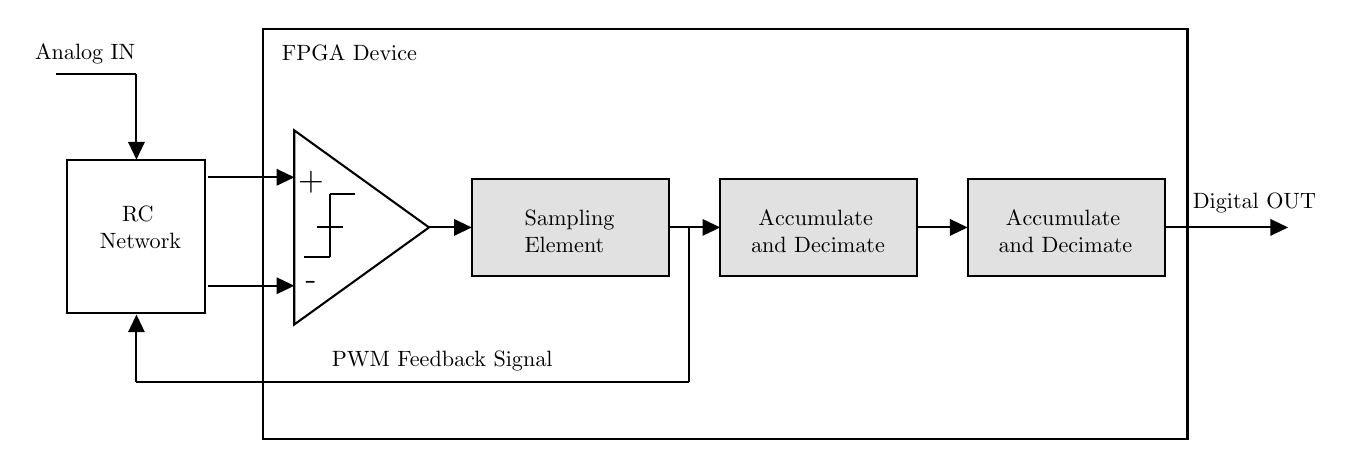
\begin{tikzpicture}[x=0.75pt,y=0.75pt,yscale=-0.95,xscale=0.95]
%uncomment if require: \path (0,300); %set diagram left start at 0, and has height of 300

%Shape: Rectangle [id:dp9604023161903008] 
\draw   (124.05,6.64) -- (593.05,6.64) -- (593.05,214.64) -- (124.05,214.64) -- cycle ;
%Straight Lines [id:da9484599770004658] 
\draw    (330.44,107.42) -- (353.05,107.42) ;
\draw [shift={(356.05,107.42)}, rotate = 180] [fill={rgb, 255:red, 0; green, 0; blue, 0 }  ][line width=0.08]  [draw opacity=0] (8.93,-4.29) -- (0,0) -- (8.93,4.29) -- cycle    ;

%Shape: Rectangle [id:dp7904328314933544] 
\draw  [fill={rgb, 255:red, 225; green, 225; blue, 225 }  ,fill opacity=1 ] (230,82.9) -- (330.05,82.9) -- (330.05,131.94) -- (230,131.94) -- cycle ;

%Straight Lines [id:da4819176246297532] 
\draw    (208.39,107.42) -- (227.05,107.42) ;
\draw [shift={(230.05,107.42)}, rotate = 180] [fill={rgb, 255:red, 0; green, 0; blue, 0 }  ][line width=0.08]  [draw opacity=0] (8.93,-4.29) -- (0,0) -- (8.93,4.29) -- cycle    ;

%Straight Lines [id:da24497687439569482] 
\draw    (60,70) -- (60,29.64) ;

\draw [shift={(60,73)}, rotate = 270] [fill={rgb, 255:red, 0; green, 0; blue, 0 }  ][line width=0.08]  [draw opacity=0] (8.93,-4.29) -- (0,0) -- (8.93,4.29) -- cycle    ;
%Straight Lines [id:da9302636844153138] 
\draw    (137.05,137) -- (96.05,137) ;

\draw [shift={(140.05,137)}, rotate = 180] [fill={rgb, 255:red, 0; green, 0; blue, 0 }  ][line width=0.08]  [draw opacity=0] (8.93,-4.29) -- (0,0) -- (8.93,4.29) -- cycle    ;
%Straight Lines [id:da2916048291189839] 
\draw    (137.05,82) -- (96.05,82) ;

\draw [shift={(140.05,82)}, rotate = 180] [fill={rgb, 255:red, 0; green, 0; blue, 0 }  ][line width=0.08]  [draw opacity=0] (8.93,-4.29) -- (0,0) -- (8.93,4.29) -- cycle    ;
%Shape: Triangle [id:dp8965603701252123] 
\draw   (208.39,107.42) -- (140.05,156.64) -- (140.05,58.2) -- cycle ;
%Shape: Rectangle [id:dp2519733387539336] 
\draw  [fill={rgb, 255:red, 225; green, 225; blue, 225 }  ,fill opacity=1 ] (356,82.9) -- (456.05,82.9) -- (456.05,131.94) -- (356,131.94) -- cycle ;

%Straight Lines [id:da7883255728251393] 
\draw    (456.44,107.42) -- (478.52,107.42) ;
\draw [shift={(481.52,107.42)}, rotate = 180] [fill={rgb, 255:red, 0; green, 0; blue, 0 }  ][line width=0.08]  [draw opacity=0] (8.93,-4.29) -- (0,0) -- (8.93,4.29) -- cycle    ;

%Shape: Rectangle [id:dp34966320633084025] 
\draw  [fill={rgb, 255:red, 225; green, 225; blue, 225 }  ,fill opacity=1 ] (481.5,82.9) -- (581.55,82.9) -- (581.55,131.94) -- (481.5,131.94) -- cycle ;

%Shape: Rectangle [id:dp20202629131702943] 
\draw   (25,73) -- (95,73) -- (95,150.64) -- (25,150.64) -- cycle ;
%Straight Lines [id:da3350824826473666] 
\draw    (19.05,29.64) -- (60,29.64) ;


%Straight Lines [id:da8160728779847974] 
\draw    (582.05,107.42) -- (641.05,107.42) ;
\draw [shift={(644.05,107.42)}, rotate = 180] [fill={rgb, 255:red, 0; green, 0; blue, 0 }  ][line width=0.08]  [draw opacity=0] (8.93,-4.29) -- (0,0) -- (8.93,4.29) -- cycle    ;

%Straight Lines [id:da4116203957240303] 
\draw    (158.05,90.27) -- (158.05,122.64) ;


%Straight Lines [id:da2244964116397019] 
\draw    (145.05,122.64) -- (158.05,122.64) ;


%Straight Lines [id:da41850801552553585] 
\draw    (158.05,90.27) -- (171.05,90.27) ;


%Straight Lines [id:da28517286500051164] 
\draw    (151.71,107.42) -- (164.71,107.42) ;


%Straight Lines [id:da7677560417405613] 
\draw    (60,154.64) -- (60,185.64) ;

\draw [shift={(60,151.64)}, rotate = 90] [fill={rgb, 255:red, 0; green, 0; blue, 0 }  ][line width=0.08]  [draw opacity=0] (8.93,-4.29) -- (0,0) -- (8.93,4.29) -- cycle    ;
%Straight Lines [id:da2763081409638619] 
\draw    (340.24,107.42) -- (340.24,185.64) ;


%Straight Lines [id:da4366815569167197] 
\draw    (340.24,185.64) -- (60,185.64) ;



% Text Node
\draw (62.05,107.42) node  [scale=0.8] [align=left] { \ \ \ RC \\Network};
% Text Node
\draw (215.05,175.14) node  [scale=0.8] [align=left] {PWM Feedback Signal};
% Text Node
\draw (168.05,19) node  [scale=0.8] [align=left] {FPGA Device};
% Text Node
\draw (279.66,109.27) node  [scale=0.8] [align=left] {Sampling\\ Element};
% Text Node
\draw (405.66,109.27) node  [scale=0.8] [align=left] { \ Accumulate\\and Decimate};
% Text Node
\draw (531.16,109.27) node  [scale=0.8] [align=left] { \ Accumulate\\and Decimate};
% Text Node
\draw (34,19.42) node  [scale=0.8] [align=left] {Analog IN};
% Text Node
\draw (627,95.05) node  [scale=0.8] [align=left] {Digital OUT};
% Text Node
\draw (148.55,84.55) node  [scale=1.2] [align=left] {+};
% Text Node
\draw (148.55,135.14) node   [align=left] {{\large -}};


\end{tikzpicture}

\caption{Schematic of the ADC obtained from Lattice\cite{LatticeADC}}
\label{adc_schematic}
\end{figure}



\subsection{PWM Regulation}
% combine with motor drive?

%\subsection{Motor Current Regulation}
The regulation of PWM limits the motor current which prevents dangerous current spikes. The measured motor current should be controlled against a predefined reference\cite{Aime}. The duty-cycle of the applied PWM can be regulated in order to control the speed of the motor\cite{Sathyan}. Duty-cycle controlled motor drive simplifies the regulation of motor speed\cite{Sathyan}.
From the specification, the PWM needs to be regulated using a simple proportional control based on the motor current. Linear regulation of PWM is a simple and efficient control system\cite{Sathyan}. 

Since the motor is being driven by a PWM signal, the current spikes up when the PWM is high and it drops when the PWM is low. In order to filter out the effect of this and get an average reading, the current should be measured in the middle of the PWM on-time. This allows the value to be averaged and provides a consistent reading.
FPGAs are able to synchronise the measurement of the current and the PWM duty-cycle in order to obtain a more accurate measurement\cite{MonmassonDesign, Gomes}. This current value is used to update the PWM value to allow for optimal control.


The PWM regulation scheme was implemented using a first-order proportional control scheme shown in Figure \ref{motor_control_loop}. 
This control scheme was chosen because it can easily be implemented in a VHDL design using a series of basic calculations and shifts. Techniques such as fixed point arithmetic can be used to implement more complex control systems. However, a first-order scheme was found to be efficient and sufficient for this application.
In this control scheme, the current value measured by the ADC is compared against the nominal value of 1A. This error is then translated into an error in PWM duty-cycle by applying a gain. Then, if the regulation is enabled in the control phase, the PWM duty-cycle value is updated. The value is truncated to ensure that it stays between the valid boundary set by the minimum and maximum values. The code which implements this PWM regulation process is shown in Appendix Item \ref{pwm-regulation-code}. The calculated value is provided to the PWM generator which translates this value into a PWM signal with a duty-cycle specified by the regulation scheme. The PWM Generator module triggers the current measurement at the midpoint of the duty-cycle in order to smooth the current measurement, as mentioned above. When triggered, the ADC value is taken in and used in the comparison. The value updates at 1kHz, once for every PWM cycle.


\begin{figure}
    \centering
    

\tikzset{every picture/.style={line width=0.75pt}} %set default line width to 0.75pt        

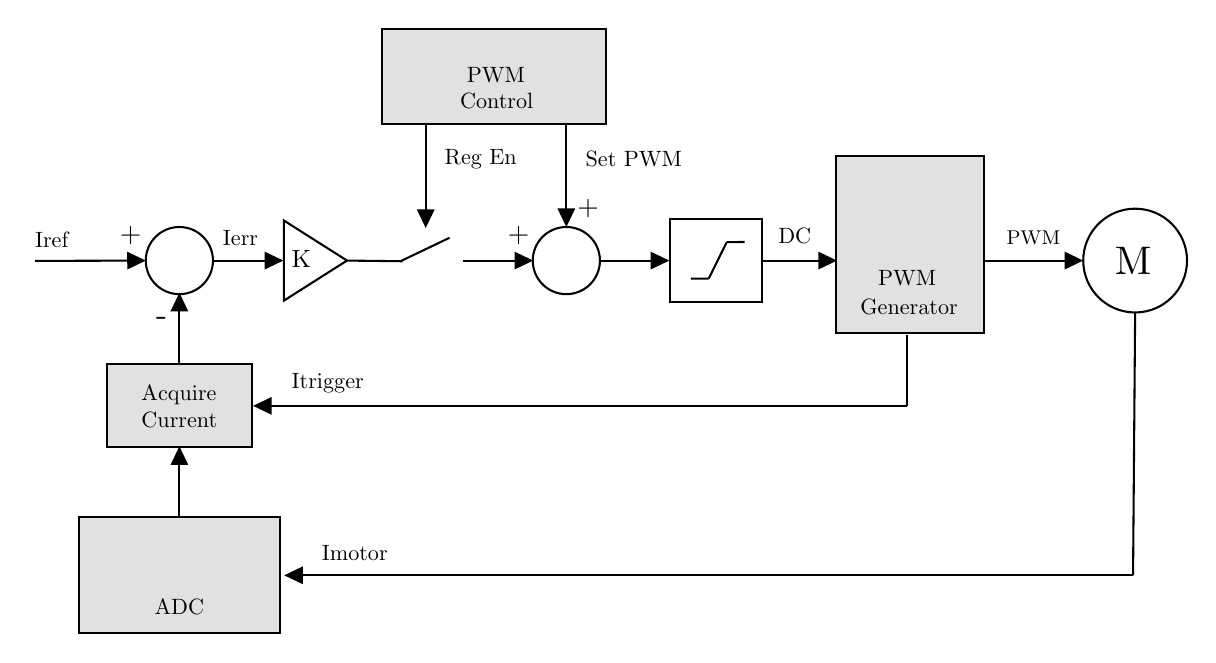
\begin{tikzpicture}[x=0.75pt,y=0.75pt,yscale=-1,xscale=1]
%uncomment if require: \path (0,300); %set diagram left start at 0, and has height of 300

%Shape: Circle [id:dp75942846606901] 
\draw   (130.33,112) .. controls (130.33,103.06) and (137.58,95.82) .. (146.52,95.82) .. controls (155.45,95.82) and (162.7,103.06) .. (162.7,112) .. controls (162.7,120.94) and (155.45,128.18) .. (146.52,128.18) .. controls (137.58,128.18) and (130.33,120.94) .. (130.33,112) -- cycle ;
%Straight Lines [id:da27986909082362965] 
\draw    (146.52,162.21) -- (146.52,130.5) ;
\draw [shift={(146.52,127.5)}, rotate = 450] [fill={rgb, 255:red, 0; green, 0; blue, 0 }  ][line width=0.08]  [draw opacity=0] (8.93,-4.29) -- (0,0) -- (8.93,4.29) -- cycle    ;

%Straight Lines [id:da6600230288463764] 
\draw    (77.05,112.16) -- (127.33,112.01) ;
\draw [shift={(130.33,112)}, rotate = 539.8299999999999] [fill={rgb, 255:red, 0; green, 0; blue, 0 }  ][line width=0.08]  [draw opacity=0] (8.93,-4.29) -- (0,0) -- (8.93,4.29) -- cycle    ;

%Shape: Rectangle [id:dp714942454713728] 
\draw  [fill={rgb, 255:red, 225; green, 225; blue, 225 }  ,fill opacity=1 ] (463,61.52) -- (534.05,61.52) -- (534.05,147) -- (463,147) -- cycle ;
%Shape: Triangle [id:dp4366865800134343] 
\draw   (227.28,112) -- (196.84,131.32) -- (196.84,92.68) -- cycle ;
%Straight Lines [id:da3696616039173719] 
\draw    (227.28,112) -- (254.05,112.32) ;


%Straight Lines [id:da9691180490319533] 
\draw    (253.71,112) -- (276.71,101) ;


%Straight Lines [id:da2520686052851293] 
\draw    (283.36,112) -- (313.98,112) ;
\draw [shift={(316.98,112)}, rotate = 180] [fill={rgb, 255:red, 0; green, 0; blue, 0 }  ][line width=0.08]  [draw opacity=0] (8.93,-4.29) -- (0,0) -- (8.93,4.29) -- cycle    ;

%Shape: Rectangle [id:dp24319017769923046] 
\draw   (382.9,92) -- (427,92) -- (427,132) -- (382.9,132) -- cycle ;
%Straight Lines [id:da7467210515424787] 
\draw    (401.56,120.66) -- (410.24,103.1) ;


%Straight Lines [id:da9410268597126219] 
\draw    (410.24,103.1) -- (418.83,103.05) ;


%Straight Lines [id:da8375418901691511] 
\draw    (392.96,120.71) -- (401.56,120.66) ;



%Straight Lines [id:da7342599903712179] 
\draw    (427.34,112) -- (460.34,112) ;
\draw [shift={(463.34,112)}, rotate = 180] [fill={rgb, 255:red, 0; green, 0; blue, 0 }  ][line width=0.08]  [draw opacity=0] (8.93,-4.29) -- (0,0) -- (8.93,4.29) -- cycle    ;

%Straight Lines [id:da296371673100567] 
\draw    (265.21,46.09) -- (265.21,93.32) ;
\draw [shift={(265.21,96.32)}, rotate = 270] [fill={rgb, 255:red, 0; green, 0; blue, 0 }  ][line width=0.08]  [draw opacity=0] (8.93,-4.29) -- (0,0) -- (8.93,4.29) -- cycle    ;

%Shape: Rectangle [id:dp9289257972427081] 
\draw  [fill={rgb, 255:red, 225; green, 225; blue, 225 }  ,fill opacity=1 ] (244.05,0.29) -- (351.94,0.29) -- (351.94,46) -- (244.05,46) -- cycle ;
%Shape: Circle [id:dp49019498566872044] 
\draw   (316.78,112) .. controls (316.78,103.06) and (324.02,95.82) .. (332.96,95.82) .. controls (341.9,95.82) and (349.14,103.06) .. (349.14,112) .. controls (349.14,120.94) and (341.9,128.18) .. (332.96,128.18) .. controls (324.02,128.18) and (316.78,120.94) .. (316.78,112) -- cycle ;
%Straight Lines [id:da140038158148579] 
\draw    (332.96,46.09) -- (332.96,92.82) ;
\draw [shift={(332.96,95.82)}, rotate = 270] [fill={rgb, 255:red, 0; green, 0; blue, 0 }  ][line width=0.08]  [draw opacity=0] (8.93,-4.29) -- (0,0) -- (8.93,4.29) -- cycle    ;

%Straight Lines [id:da6535254105925976] 
\draw    (162.96,112) -- (193.58,112) ;
\draw [shift={(196.58,112)}, rotate = 180] [fill={rgb, 255:red, 0; green, 0; blue, 0 }  ][line width=0.08]  [draw opacity=0] (8.93,-4.29) -- (0,0) -- (8.93,4.29) -- cycle    ;

%Straight Lines [id:da8262984100189177] 
\draw    (348.94,112) -- (379.55,112) ;
\draw [shift={(382.55,112)}, rotate = 180] [fill={rgb, 255:red, 0; green, 0; blue, 0 }  ][line width=0.08]  [draw opacity=0] (8.93,-4.29) -- (0,0) -- (8.93,4.29) -- cycle    ;

%Shape: Circle [id:dp25249517388379217] 
\draw   (582,112) .. controls (582,98.19) and (593.19,87) .. (607,87) .. controls (620.81,87) and (632,98.19) .. (632,112) .. controls (632,125.81) and (620.81,137) .. (607,137) .. controls (593.19,137) and (582,125.81) .. (582,112) -- cycle ;

%Straight Lines [id:da6638712668031186] 
\draw    (534.34,112) -- (579,112) ;
\draw [shift={(582,112)}, rotate = 180] [fill={rgb, 255:red, 0; green, 0; blue, 0 }  ][line width=0.08]  [draw opacity=0] (8.93,-4.29) -- (0,0) -- (8.93,4.29) -- cycle    ;

%Shape: Rectangle [id:dp6025687451357558] 
\draw  [fill={rgb, 255:red, 225; green, 225; blue, 225 }  ,fill opacity=1 ] (111.52,162) -- (181.52,162) -- (181.52,202) -- (111.52,202) -- cycle ;
%Shape: Rectangle [id:dp6368460798569435] 
\draw  [fill={rgb, 255:red, 225; green, 225; blue, 225 }  ,fill opacity=1 ] (98.03,235.64) -- (195,235.64) -- (195,291.64) -- (98.03,291.64) -- cycle ;
%Straight Lines [id:da3095935870834763] 
\draw    (146.52,236.21) -- (146.52,204.5) ;
\draw [shift={(146.52,201.5)}, rotate = 450] [fill={rgb, 255:red, 0; green, 0; blue, 0 }  ][line width=0.08]  [draw opacity=0] (8.93,-4.29) -- (0,0) -- (8.93,4.29) -- cycle    ;

%Straight Lines [id:da7119757417617545] 
\draw    (497.15,182) -- (185.05,182) ;
\draw [shift={(182.05,182)}, rotate = 360] [fill={rgb, 255:red, 0; green, 0; blue, 0 }  ][line width=0.08]  [draw opacity=0] (8.93,-4.29) -- (0,0) -- (8.93,4.29) -- cycle    ;

%Straight Lines [id:da555961758391875] 
\draw    (606,263.64) -- (200.05,263.64) ;
\draw [shift={(197.05,263.64)}, rotate = 360] [fill={rgb, 255:red, 0; green, 0; blue, 0 }  ][line width=0.08]  [draw opacity=0] (8.93,-4.29) -- (0,0) -- (8.93,4.29) -- cycle    ;

%Straight Lines [id:da5618757081316239] 
\draw    (606,263.64) -- (607,137) ;


%Straight Lines [id:da9238020071399877] 
\draw    (497.15,182) -- (497.15,147.64) ;



% Text Node
\draw (123,100.16) node  [scale=1] [align=left] {+};
% Text Node
\draw (138.02,140) node  [scale=1.2] [align=left] {\mbox{-}};
% Text Node
\draw (85,102) node  [scale=0.8] [align=left] {Iref};
% Text Node
\draw (205.21,111) node  [scale=0.9] [align=left] {K};
% Text Node
\draw (497.15,120.52) node  [scale=0.8] [align=left] {PWM};
% Text Node
\draw (498.1,134.52) node  [scale=0.8] [align=left] {Generator};
% Text Node
\draw (299.42,35.09) node  [scale=0.8] [align=left] {Control};
% Text Node
\draw (298.99,22.49) node  [scale=0.8] [align=left] {PWM};
% Text Node
\draw (558,101.16) node  [scale=0.8] [align=left] {{\small PWM}};
% Text Node
\draw (606,112) node  [scale=1.44] [align=left] {M};
% Text Node
\draw (443,100) node  [scale=0.8] [align=left] {DC};
% Text Node
\draw (146.52,182.33) node  [scale=0.8] [align=left] {Acquire\\Current};
% Text Node
\draw (146.52,279) node  [scale=0.8] [align=left] {ADC};
% Text Node
\draw (310,100.16) node  [scale=1] [align=left] {+};
% Text Node
\draw (343.46,87.16) node  [scale=1] [align=left] {+};
% Text Node
\draw (365.46,63) node  [scale=0.8] [align=left] {Set PWM};
% Text Node
\draw (291.71,63) node  [scale=0.8] [align=left] {Reg En};
% Text Node
\draw (176,101.16) node  [scale=0.8] [align=left] {Ierr};
% Text Node
\draw (218,171) node  [scale=0.8] [align=left] {Itrigger};
% Text Node
\draw (231.02,252.64) node  [scale=0.8] [align=left] {Imotor};


\end{tikzpicture}

    \caption{PWM regulation process control loop}
    \label{motor_control_loop}
\end{figure}

This control scheme was used to map to the response from the microcontroller-based regulation scheme. The output of the regulation scheme was analysed and modelled. The microcontroller output that was analysed and modelled is shown in Section \ref{regulation-results}. It was found to be a simple proportional controller. The simple control response was modified to include processes outlined in the requirements. For example, the current is acquired half-way through the on-time using a trigger from the PWM duty-cycle. Truncation was performed on the calculated value to ensure that it stayed between the defined minimum and the calculated maximum.

\subsection{Motor Driving}

The motor is driven using an H-bridge scheme consisting of two IGBT and Thyristor pairs. This circuit can be seen in Figure \ref{motor_control_circuit}. The motor drive module has to multiplex the PWM and control signals generated by the regulation phase to drive the correct IGBTs and Thyristors. The driving sequence is being modelled on the current set of requirements. It contains several discrete stages in order to drive the Thyristors and IGBTs to move the motor to the required position.

\begin{figure}
\centering


\tikzset{every picture/.style={line width=0.75pt}} %set default line width to 0.75pt        

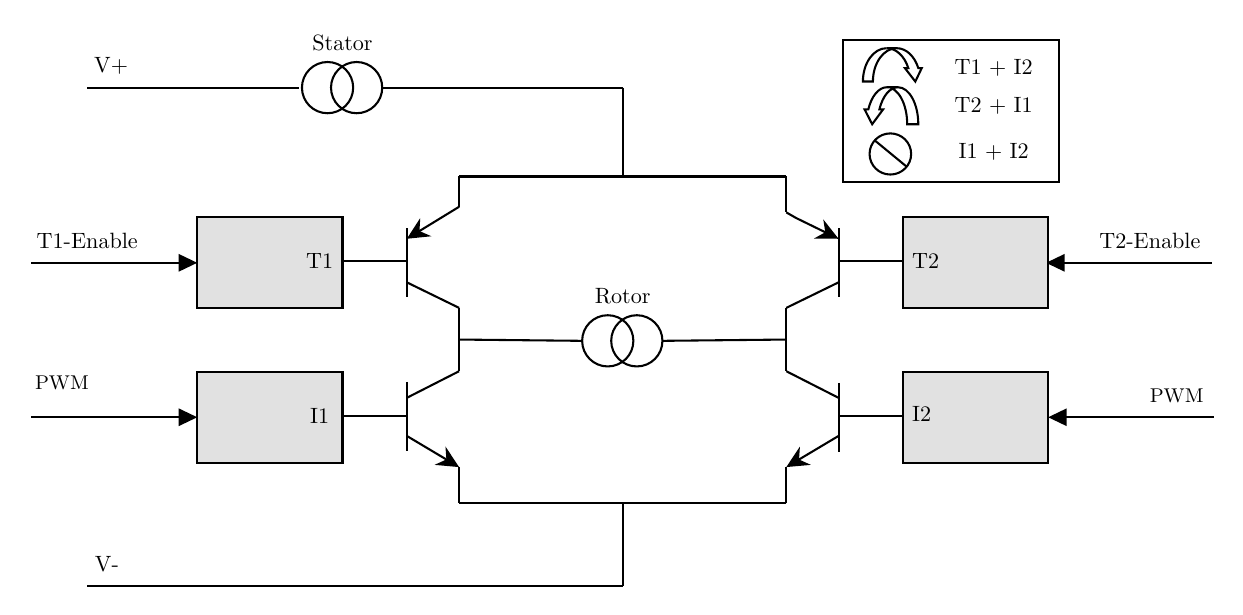
\begin{tikzpicture}[x=0.75pt,y=0.75pt,yscale=-1,xscale=1]
%uncomment if require: \path (0,300); %set diagram left start at 0, and has height of 300

%Straight Lines [id:da9221466297195395] 
\draw    (189.05,188.5) -- (158.05,188.5) ;


%Straight Lines [id:da5673743870695822] 
\draw    (8.05,114.59) -- (85.05,114.59) ;
\draw [shift={(88.05,114.59)}, rotate = 180] [fill={rgb, 255:red, 0; green, 0; blue, 0 }  ][line width=0.08]  [draw opacity=0] (8.93,-4.29) -- (0,0) -- (8.93,4.29) -- cycle    ;

%Straight Lines [id:da5344017083576562] 
\draw    (8.05,189) -- (85.05,189) ;
\draw [shift={(88.05,189)}, rotate = 180] [fill={rgb, 255:red, 0; green, 0; blue, 0 }  ][line width=0.08]  [draw opacity=0] (8.93,-4.29) -- (0,0) -- (8.93,4.29) -- cycle    ;

%Straight Lines [id:da4468699428839338] 
\draw    (214.22,73) -- (214.22,87.6) ;


%Straight Lines [id:da26254747962825764] 
\draw    (214.22,87.6) -- (191.6,101.43) ;
\draw [shift={(189.05,103)}, rotate = 328.53999999999996] [fill={rgb, 255:red, 0; green, 0; blue, 0 }  ][line width=0.08]  [draw opacity=0] (10.72,-5.15) -- (0,0) -- (10.72,5.15) -- (7.12,0) -- cycle    ;

%Straight Lines [id:da5823961798906938] 
\draw    (428.05,188.5) -- (397.05,188.5) ;


%Straight Lines [id:da29909831649241614] 
\draw    (428.05,113.5) -- (397.05,113.5) ;


%Straight Lines [id:da2356065415871993] 
\draw    (189.05,113.5) -- (158.05,113.5) ;


%Straight Lines [id:da30663699958544943] 
\draw    (189.05,98) -- (189.05,131.18) ;


%Straight Lines [id:da31696707767211185] 
\draw    (397.05,98) -- (397.05,131.18) ;


%Straight Lines [id:da673348118293702] 
\draw    (500.05,114.59) -- (577.05,114.59) ;

\draw [shift={(497.05,114.59)}, rotate = 0] [fill={rgb, 255:red, 0; green, 0; blue, 0 }  ][line width=0.08]  [draw opacity=0] (8.93,-4.29) -- (0,0) -- (8.93,4.29) -- cycle    ;
%Straight Lines [id:da3029592242109622] 
\draw    (501.05,189) -- (578.05,189) ;

\draw [shift={(498.05,189)}, rotate = 0] [fill={rgb, 255:red, 0; green, 0; blue, 0 }  ][line width=0.08]  [draw opacity=0] (8.93,-4.29) -- (0,0) -- (8.93,4.29) -- cycle    ;
%Straight Lines [id:da8114410961824066] 
\draw    (371.87,90.3) -- (376.68,93.04) -- (394.35,101.68) ;
\draw [shift={(397.05,103)}, rotate = 206.07] [fill={rgb, 255:red, 0; green, 0; blue, 0 }  ][line width=0.08]  [draw opacity=0] (10.72,-5.15) -- (0,0) -- (10.72,5.15) -- (7.12,0) -- cycle    ;

%Straight Lines [id:da20108401284003996] 
\draw    (371.87,73) -- (371.87,90.3) ;


%Straight Lines [id:da8481295471076566] 
\draw    (371.87,73) -- (214.22,73) ;


%Shape: Circle [id:dp10268436833983152] 
\draw   (273.51,152.18) .. controls (273.51,145.37) and (279.03,139.84) .. (285.85,139.84) .. controls (292.66,139.84) and (298.19,145.37) .. (298.19,152.18) .. controls (298.19,159) and (292.66,164.52) .. (285.85,164.52) .. controls (279.03,164.52) and (273.51,159) .. (273.51,152.18) -- cycle ;
%Shape: Circle [id:dp39801516955430727] 
\draw   (287.51,152.18) .. controls (287.51,145.37) and (293.03,139.84) .. (299.85,139.84) .. controls (306.66,139.84) and (312.19,145.37) .. (312.19,152.18) .. controls (312.19,159) and (306.66,164.52) .. (299.85,164.52) .. controls (293.03,164.52) and (287.51,159) .. (287.51,152.18) -- cycle ;

%Straight Lines [id:da726831823671015] 
\draw    (189.05,124) -- (214.22,136.3) ;


%Straight Lines [id:da778435519184604] 
\draw    (371.87,136.3) -- (397.05,124) ;


%Straight Lines [id:da4015757785120837] 
\draw    (189.05,171.91) -- (189.05,205.09) ;


%Straight Lines [id:da23166080135755474] 
\draw    (397.05,172.41) -- (397.05,205.59) ;


%Straight Lines [id:da7946452898081748] 
\draw    (189.05,179.64) -- (214.22,166.82) ;


%Straight Lines [id:da2217710859730495] 
\draw    (371.87,166.82) -- (397.05,179.64) ;


%Straight Lines [id:da5050058101228307] 
\draw    (214.22,136.3) -- (214.22,166.82) ;


%Straight Lines [id:da07368058014858048] 
\draw    (371.87,136.3) -- (371.87,166.82) ;


%Straight Lines [id:da4463883229770369] 
\draw    (214.22,151.56) -- (273.51,152.18) ;


%Straight Lines [id:da606524752619622] 
\draw    (312.19,152.18) -- (371.87,151.56) ;


%Straight Lines [id:da43391584718083376] 
\draw    (189.05,198) -- (211.64,211.46) ;
\draw [shift={(214.22,213)}, rotate = 210.79] [fill={rgb, 255:red, 0; green, 0; blue, 0 }  ][line width=0.08]  [draw opacity=0] (10.72,-5.15) -- (0,0) -- (10.72,5.15) -- (7.12,0) -- cycle    ;

%Straight Lines [id:da6840402308453948] 
\draw    (397.05,198) -- (374.45,211.46) ;
\draw [shift={(371.87,213)}, rotate = 329.21000000000004] [fill={rgb, 255:red, 0; green, 0; blue, 0 }  ][line width=0.08]  [draw opacity=0] (10.72,-5.15) -- (0,0) -- (10.72,5.15) -- (7.12,0) -- cycle    ;

%Straight Lines [id:da14157911992399308] 
\draw    (371.87,230.3) -- (214.22,230.3) ;


%Straight Lines [id:da9684058826846] 
\draw    (371.87,213) -- (371.87,230.3) ;


%Straight Lines [id:da027240572979521538] 
\draw    (214.22,213) -- (214.22,230.3) ;


%Shape: Circle [id:dp751541628776144] 
\draw   (138.51,30.18) .. controls (138.51,23.37) and (144.03,17.84) .. (150.85,17.84) .. controls (157.66,17.84) and (163.19,23.37) .. (163.19,30.18) .. controls (163.19,37) and (157.66,42.52) .. (150.85,42.52) .. controls (144.03,42.52) and (138.51,37) .. (138.51,30.18) -- cycle ;
%Shape: Circle [id:dp12782068359122056] 
\draw   (152.51,30.18) .. controls (152.51,23.37) and (158.03,17.84) .. (164.85,17.84) .. controls (171.66,17.84) and (177.19,23.37) .. (177.19,30.18) .. controls (177.19,37) and (171.66,42.52) .. (164.85,42.52) .. controls (158.03,42.52) and (152.51,37) .. (152.51,30.18) -- cycle ;

%Straight Lines [id:da9745722307494478] 
\draw    (293.05,30.18) -- (177.19,30.18) ;


%Straight Lines [id:da9525535594657324] 
\draw    (293.05,30.18) -- (293.05,73) ;


%Straight Lines [id:da7344305010710814] 
\draw    (137.05,30.18) -- (35.05,30.18) ;


%Straight Lines [id:da5373673836671371] 
\draw    (293.05,270.18) -- (35.05,270.18) ;


%Straight Lines [id:da8535356105812089] 
\draw    (293.05,230.3) -- (293.05,270.18) ;


%Curve Right Arrow [id:dp07248280783179872] 
\draw  [fill={rgb, 255:red, 255; green, 255; blue, 255 }  ,fill opacity=1 ] (425.02,11.18) .. controls (418.72,11.18) and (413.6,18.38) .. (413.6,27.25) -- (408.78,27.25) .. controls (408.78,18.38) and (413.89,11.18) .. (420.2,11.18) ;\draw  [fill={rgb, 255:red, 255; green, 255; blue, 255 }  ,fill opacity=1 ] (420.2,11.18) .. controls (424.88,11.18) and (428.9,15.15) .. (430.67,20.83) -- (429.06,20.83) -- (434.03,27.25) -- (437.1,20.83) -- (435.49,20.83) .. controls (433.73,15.15) and (429.7,11.18) .. (425.02,11.18)(420.2,11.18) -- (425.02,11.18) ;
%Curve Left Arrow [id:dp35549290685095736] 
\draw  [fill={rgb, 255:red, 255; green, 255; blue, 255 }  ,fill opacity=1 ] (425.68,30) .. controls (431.08,30) and (435.46,37.98) .. (435.46,47.82) -- (430.11,47.82) .. controls (430.11,37.98) and (425.74,30) .. (420.34,30) ;\draw  [fill={rgb, 255:red, 255; green, 255; blue, 255 }  ,fill opacity=1 ] (420.34,30) .. controls (416.33,30) and (412.89,34.4) .. (411.38,40.69) -- (409.6,40.69) -- (413.24,47.82) -- (418.51,40.69) -- (416.72,40.69) .. controls (418.23,34.4) and (421.68,30) .. (425.68,30)(420.34,30) -- (425.68,30) ;
%Shape: Ellipse [id:dp4400378009685477] 
\draw   (411.99,62.15) .. controls (411.99,56.67) and (416.47,52.24) .. (422,52.24) .. controls (427.53,52.24) and (432.02,56.67) .. (432.02,62.15) .. controls (432.02,67.62) and (427.53,72.06) .. (422,72.06) .. controls (416.47,72.06) and (411.99,67.62) .. (411.99,62.15) -- cycle ;
%Straight Lines [id:da593928177084287] 
\draw    (414.32,55.48) -- (429.89,68.29) ;


%Shape: Rectangle [id:dp9415861976749436] 
\draw   (399.03,7.25) -- (503.05,7.25) -- (503.05,75.64) -- (399.03,75.64) -- cycle ;
%Shape: Rectangle [id:dp9348588765520855] 
\draw  [fill={rgb, 255:red, 225; green, 225; blue, 225 }  ,fill opacity=1 ] (88.05,92.73) -- (158.05,92.73) -- (158.05,136.45) -- (88.05,136.45) -- cycle ;
%Shape: Rectangle [id:dp09631198686380071] 
\draw  [fill={rgb, 255:red, 225; green, 225; blue, 225 }  ,fill opacity=1 ] (428.05,167.14) -- (498.05,167.14) -- (498.05,210.86) -- (428.05,210.86) -- cycle ;
%Shape: Rectangle [id:dp45121828009239695] 
\draw  [fill={rgb, 255:red, 225; green, 225; blue, 225 }  ,fill opacity=1 ] (428.05,92.73) -- (498.05,92.73) -- (498.05,136.45) -- (428.05,136.45) -- cycle ;
%Shape: Rectangle [id:dp41843258071231526] 
\draw  [fill={rgb, 255:red, 225; green, 225; blue, 225 }  ,fill opacity=1 ] (88.05,167.14) -- (158.05,167.14) -- (158.05,210.86) -- (88.05,210.86) -- cycle ;

% Text Node
\draw (559.94,178.5) node  [scale=0.8] [align=left] {{\small PWM}};
% Text Node
\draw (547.05,104.09) node  [scale=0.8] [align=left] {T2-Enable};
% Text Node
\draw (22.87,172.5) node  [scale=0.8] [align=left] {{\small PWM}};
% Text Node
\draw (35.05,104.09) node  [scale=0.8] [align=left] {T1-Enable};
% Text Node
\draw (147.05,113.5) node  [scale=0.8] [align=left] {T1};
% Text Node
\draw (439.05,113.5) node  [scale=0.8] [align=left] {T2};
% Text Node
\draw (147.05,188.5) node  [scale=0.8] [align=left] {I1};
% Text Node
\draw (437.05,187.5) node  [scale=0.8] [align=left] {I2};
% Text Node
\draw (46.55,19.68) node  [scale=0.8] [align=left] {V+};
% Text Node
\draw (44.55,259.68) node  [scale=0.8] [align=left] {V-};
% Text Node
\draw (293.05,130.5) node  [scale=0.8] [align=left] {Rotor};
% Text Node
\draw (158.05,8.5) node  [scale=0.8] [align=left] {Stator};
% Text Node
\draw (471.78,20.52) node  [scale=0.8] [align=left] {T1 + I2};
% Text Node
\draw (471.78,39.17) node  [scale=0.8] [align=left] {T2 + I1};
% Text Node
\draw (471.78,61.17) node  [scale=0.8] [align=left] {I1 + I2};


\end{tikzpicture}

\caption{Motor driving circuit diagram showing a pair of Thyristors (T1 and T2) and a pair of IGBTs (I1 and I2) redrawn from the ATyS specification (requirements: Drive R1 and Drive R2)}
\label{motor_control_circuit}
\end{figure}

%Design considerations for motor drives include providing stable speed control and preventing large currents\cite{Bodur}.

Indicated in the diagram (Figure \ref{motor_control_circuit}) are the control signals required to perform certain actions on the motor. This includes the direction of rotation which is achieved by stimulating opposite Thyristor and IGBT combinations. Additionally, the brake functionality is shown which involves driving both of the IGBTs. The PWM from the regulation scheme is provided to the correct IGBT by the Motor Driving module. The code which provides the necessary control to the IGBTs is shown in Appendix Item \ref{igbt-driving-code}.

\subsection{Clock Design}

As defined in the micro-processor specification, the requirement for the PWM produced is a 1kHz PWM signal with a resolution of 100. This means that the PWM can be controlled to an accuracy of 1\%. From this, it can be determined that the PWM must be driven with a clock of at least 100kHz. The ADC requires a higher clock frequency in order to perform oversampling. The speed of the ADC determines the accuracy of the measurement used in current regulation. Therefore, the faster the result of the ADC is produced, the better. Due to the ADC implementation, this metric translates directly to the clock frequency. 

The internal oscillator on the MachXO2 was used to generate the higher clock for the ADC. The maximum value of the clock, 133 MHz, was used in order to maximise the data-rate of the current measurements. This clock signal was divided down to 200kHz using the phase-locked loop in order to drive the rest of the system. This is sufficient to allow for the regulation process to update the PWM before the next cycle. It also allows for the PWM signal to have double the resolution than is specified.

\subsection{Diagnostics}
\label{diagnostic-section}
System diagnostics are highly recommended by the IEC 61508 SIL standards as a measure to reduce the effect of errors\cite{IEC61508}. They help to improve the functional safety of a device by detecting, and possibly correcting, dangerous conditions\cite{Jeppesen}. Where good design practices can prevent systematic errors in the system, diagnostics help to prevent and reduce the effect of random hardware faults. The implementation of diagnostics for this system is beyond the scope of this project. A number of applicable diagnostics are discussed in the remainder of this section.


A number of diagnostics are discussed by Jeppesen, Rajamani and Smith\cite{Jeppesen}. Diagnostics which have been applied to the FPGA solutions include a PWM checker, watchdog timer, ADC out-of-range detection and module self-tests by error injection\cite{Jeppesen}.
Each of these diagnostic measures could be applied to the ATyS processor developed in this project to enhance the functional safety of the solution.

Additionally, full redundancy architectures can be utilised in order to verify system behaviour\cite{Jeppesen, BorcsokDesign}. The use of a redundancy architecture, which is possible in FPGAs\cite{HayekSRAM}, is recommended by the standards\cite{IEC61508, Borcsok} as it increases the reliability of the system\cite{HayekSafety}. Duplex redundancy is a common methodology which requires the system to be synthesised twice and the outputs are compared\cite{HayekSRAM}. An example duplex redundancy architecture, 1oo2 (one out of two), is shown in Figure \ref{onchip_redundancy}. The system must be synthesised twice in order to compare the results and ensure that the results are consistent as shown in the diagram.



\begin{figure}
    \centering
    

\tikzset{every picture/.style={line width=0.75pt}} %set default line width to 0.75pt        

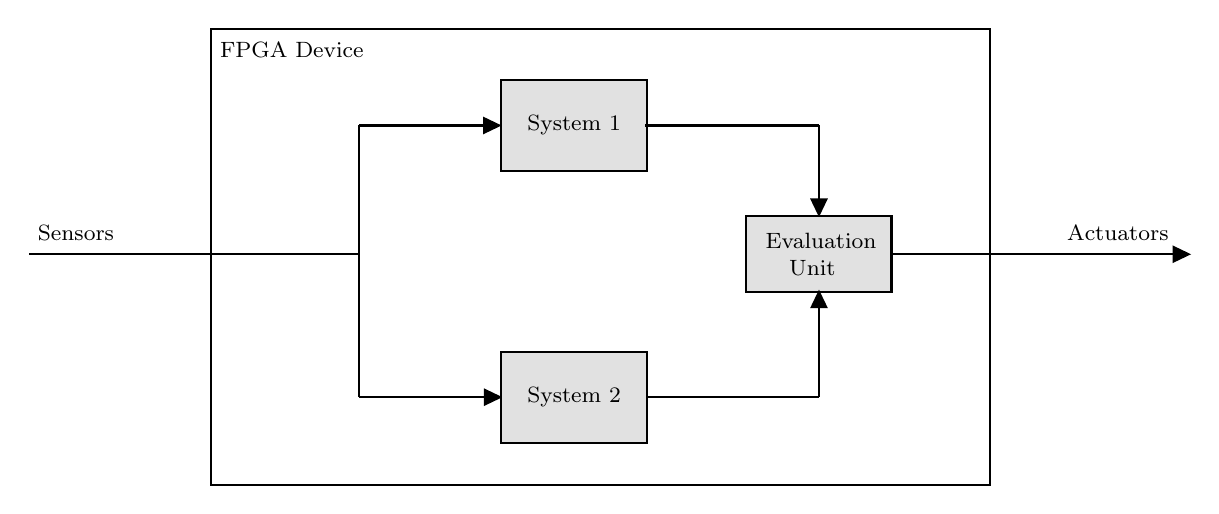
\begin{tikzpicture}[x=0.75pt,y=0.75pt,yscale=-1,xscale=1]
%uncomment if require: \path (0,300); %set diagram left start at 0, and has height of 300

%Straight Lines [id:da5881950910157023] 
\draw    (286.51,183) -- (220.3,183) ;

\draw [shift={(289.51,183)}, rotate = 180] [fill={rgb, 255:red, 0; green, 0; blue, 0 }  ][line width=0.08]  [draw opacity=0] (8.93,-4.29) -- (0,0) -- (8.93,4.29) -- cycle    ;
%Straight Lines [id:da25338917902177904] 
\draw    (220.3,52.09) -- (220.3,183) ;


%Shape: Rectangle [id:dp3450500434713657] 
\draw  [fill={rgb, 255:red, 225; green, 225; blue, 225 }  ,fill opacity=1 ] (289.05,161.14) -- (359.05,161.14) -- (359.05,204.86) -- (289.05,204.86) -- cycle ;
%Shape: Rectangle [id:dp14922514498310435] 
\draw  [fill={rgb, 255:red, 225; green, 225; blue, 225 }  ,fill opacity=1 ] (289.05,30.23) -- (359.05,30.23) -- (359.05,73.95) -- (289.05,73.95) -- cycle ;
%Straight Lines [id:da0868762150769582] 
\draw    (286.12,52.09) -- (220.3,52.09) ;

\draw [shift={(289.12,52.09)}, rotate = 180] [fill={rgb, 255:red, 0; green, 0; blue, 0 }  ][line width=0.08]  [draw opacity=0] (8.93,-4.29) -- (0,0) -- (8.93,4.29) -- cycle    ;
%Straight Lines [id:da9680613737529542] 
\draw    (220.3,114.14) -- (61.3,114.14) ;


%Shape: Rectangle [id:dp2265192536845475] 
\draw  [fill={rgb, 255:red, 225; green, 225; blue, 225 }  ,fill opacity=1 ] (407.1,95.86) -- (476.99,95.86) -- (476.99,132.42) -- (407.1,132.42) -- cycle ;
%Straight Lines [id:da668687133025897] 
\draw    (442.05,134.2) -- (442.05,183) ;

\draw [shift={(442.05,131.2)}, rotate = 90] [fill={rgb, 255:red, 0; green, 0; blue, 0 }  ][line width=0.08]  [draw opacity=0] (8.93,-4.29) -- (0,0) -- (8.93,4.29) -- cycle    ;
%Straight Lines [id:da3164126413280457] 
\draw    (442.05,93.2) -- (442.05,52.09) ;

\draw [shift={(442.05,96.2)}, rotate = 270] [fill={rgb, 255:red, 0; green, 0; blue, 0 }  ][line width=0.08]  [draw opacity=0] (8.93,-4.29) -- (0,0) -- (8.93,4.29) -- cycle    ;
%Straight Lines [id:da2018473186011438] 
\draw    (442.05,183) -- (359.3,183) ;


%Straight Lines [id:da8685031016449603] 
\draw    (442.05,52.09) -- (358.3,52.09) ;


%Straight Lines [id:da7841339318502909] 
\draw    (618.3,114.14) -- (477.3,114.14) ;

\draw [shift={(621.3,114.14)}, rotate = 180] [fill={rgb, 255:red, 0; green, 0; blue, 0 }  ][line width=0.08]  [draw opacity=0] (8.93,-4.29) -- (0,0) -- (8.93,4.29) -- cycle    ;
%Shape: Rectangle [id:dp3914738316121473] 
\draw   (149.3,5.47) -- (524.3,5.47) -- (524.3,225.2) -- (149.3,225.2) -- cycle ;

% Text Node
\draw (324.05,52.09) node  [font=\footnotesize] [align=left] {System 1};
% Text Node
\draw (324.05,183) node  [font=\footnotesize] [align=left] {System 2};
% Text Node
\draw (443.05,114.14) node  [font=\footnotesize] [align=left] {Evaluation\\ \ \ \ Unit};
% Text Node
\draw (586.05,103.64) node  [font=\footnotesize] [align=left] {Actuators};
% Text Node
\draw (84.05,103.64) node  [font=\footnotesize] [align=left] {Sensors};
% Text Node
\draw (188.05,15.59) node  [font=\footnotesize] [align=left] {FPGA Device};


\end{tikzpicture}

    \caption{FPGA (1oo2) on-chip redundancy architecture (based on diagram in \cite{Borcsok})}
    \label{onchip_redundancy}
\end{figure}

%\begin{figure}[h]
%\centering
%\includegraphics[width=0.89\textwidth]{images/SystemRedundan%cyInFPGAs.pdf}
%\caption{FPGA On-chip Redundancy 1oo2 Architecture\cite{Borcsok}}
%\label{onchip_redundancy}
%\end{figure}

%Artihmetic operations should be avoided in favour of logical operations to allow for efficient synthesis\cite{deCastro}. Transitioning algorithms and functionality requires a redesign in order to realise the benefits of an FPGA implementation\cite{deCastro}.

\section{Physical Prototype}
As part of the development of this project, a physical prototype was created. The prototype consists of a modified version of the PCB used in the microcontroller solution. In this section, the adoption of tools and components used in the implementation of the prototype are discussed. The PCB changes, made by the Socomec design team, in order to incorporate an FPGA into the existing commercial ATyS PCB are also discussed in this section. The results of the synthesis process for the design are presented. Additionally, the implemented behaviour of the prototype is presented.

\subsection{FPGA and Tool Adoption}

A number of factors need to be considered in the selection of an embedded controller. These include cost, size, performance, availability and verification capability\cite{Gomes}. The FPGA which has been adopted for the project is the Lattice Mach XO2-2000. This FPGA has 2112 LUT4 logic units. The larger package was chosen to provide as much flexibility as possible for the prototype. The MachXO2 FPGA has in-built diagnostics including configuration checks. The safety compatible version of Lattice Diamond (Lattice Diamond 2.0) was used for the development in this project. The safety standards require proven-in-use tools to be used in the development of safety-critical systems. This version of Diamond has been marked as proven-in-use by Lattice.


\subsection{PCB Re-design}

\begin{figure}[h]
\centering
\includegraphics[width=0.89\textwidth]{images/PrototypeBoard.pdf}
\caption{The prototype motor control PCB with an FPGA processor}
\label{board}
\end{figure}

The PCB was re-designed to allow for the prototyping of an FPGA solution. This PCB can be seen in Figure \ref{board}. This task was performed by design engineers at Socomec. The movement to an FPGA solution required minimal changes to the existing design. The most considerable change was the switch of the FPGA in the place of the microcontroller. Since most of the FPGA pins are freely configurable, the change from a microcontroller to an FPGA is flexible in terms of routing\cite{SalewskiSystematic}. The nature of the design implementation allowed the ADC to be implemented using a simple RC network. External memory units could be removed as the FPGA has internal memory units. A JTAG programming interface was added to the design to allow the FPGA to be reprogrammed.

\subsection{Prototyping Strategy}
\label{prototyping-strategy}
An incremental prototyping strategy was used in order to test each of the design modules independently. This involved mapping inputs to the series of push-buttons used for position acquisition and mapping the outputs to general I/O ports. This allowed the inputs of modules to be simulated and the outputs to be analysed on an oscilloscope. This provided insight into the physical behaviour of each module and allowed the design to be implemented incrementally. This process was performed after the module verification, discussed in  Section \ref{verification}. This meant that each of the individual modules had already been verified which resulted in a rapid implementation process with each of the modules working as expected. 

Despite the fact that each of the modules had been functionally verified, there were a number of problems relating to the specification which were identified while prototyping the design. For example, the naming convention was inconsistent between the schematic for the microcontroller solution and the FPGA board. This resulted in the positions being read in reverse. For example, position 1 was read as position 2. However, direction calculation and the position translation was updated and the expected behaviour was realised.

Components which were not utilised by the prototype were used as debugging interfaces. The interface used to communicate with the second control board was used to view the values produced by the ADC. This allowed the RC components to be tuned to the optimum range for the measurement voltage. It also allowed for debugging when testing the regulation control process as the values could be stepped through on the oscilloscope and the response could be analysed.

\subsection{Synthesis Results}

Mach XO2 FPGAs come in different package sizes for which the number of logic units and the number of pins varies as well as the cost. The synthesised prototype design used 36\% of the capacity of the Mach XO2-2000 FPGA used in the project. This leaves 1352 of the 2112 logic units in the FPGA available for use. This additional space could be used for the diagnostic components and redundancy architectures discussed in Section \ref{diagnostic-section}. Alternatively, the package size could be reduced. The design used 20 of the
100 FPGA I/O ports. This was composed of eight for the position measurement, three for the command input, three for each of the ADC measurements and six for the motor control signals.

\subsection{Prototype Behaviour}
The prototype successfully implemented the safety function of the device. Physical prototyping allowed for the behaviour of the designed system to be verified and compared against the existing solution. Functionality of the physical prototype includes performing the core safety function of the device, performing a transfer from one power source to another. This behaviour requires the correct acquisition of commands and position and calculation  of the required movement as well as the translation of this into a control sequence to drive the motor. Additional functionality includes the regulation of the current in order to control the response in cases of stalled or blocked motors. The timeout and movement retry behaviour in the microcontroller solution was also replicated in the design and prototype.

\section{Design Conclusion}

The FPGA-based system was designed based on the original microcontroller-based system specification. The motor control behaviour was identified as the safety function of the device. The requirements that allow this to be performed were derived from this specification and became the requirements for the design of the FPGA system. Following the V-model process, a system architecture was derived from these requirements. Four main system processes were identified in order to meet the requirements and were integrated as modules to form the system architecture. These modules are Input Processing, ADC, PWM Regulation and Motor Driving. The design and implementation of these modules has been described in this section. Additionally, the clock design was discussed. The planning of diagnostics was also presented; however, the implementation of these diagnostics was outside the scope of the project. Finally, the physical prototype which was created as part of the development in this project was presented in this section. The prototype successfully replicated the safety function behaviour of the microcontroller board in the ATyS.